%%
%% licence       kaneton licence
%%
%% project       kaneton
%%
%% file          /home/mycure/kaneton/view/papers/assignments/assignments.tex
%%
%% created       julien quintard   [wed dec  7 16:53:52 2005]
%% updated       julien quintard   [thu jan  5 08:50:11 2006]
%%

%
% template
%

%
% ---------- header -----------------------------------------------------------
%
% project       kaneton
%
% license       kaneton
%
% file          /home/mycure/kaneton/view/template/paper.tex
%
% created       julien quintard   [wed may 16 18:17:37 2007]
% updated       julien quintard   [fri oct  5 07:00:45 2007]
%

%
% class
%

\documentclass[10pt,a4wide]{article}

%
% packages
%

\usepackage[english]{babel}
\usepackage[T1]{fontenc}
\usepackage{a4wide}
\usepackage{fancyheadings}
\usepackage{multicol}
\usepackage{indentfirst}
\usepackage{graphicx}
\usepackage{color}
\usepackage{xcolor}
\usepackage{verbatim}
\usepackage{aeguill}

\pagestyle{fancy}

\setlength{\footrulewidth}{0.3pt}
\setlength{\parindent}{0.3cm}
\setlength{\parskip}{2ex plus 0.5ex minus 0.2ex}

%
% logos
%

\newcommand{\logos}
  {
    \begin{center}
      
\includegraphics[scale=0.8]{\path/logo/kaneton.pdf}
    \end{center}
  }

%
% prototype
%

\newcommand\prototype[2]{
  \begin{tabular}{p{0.2cm}p{13.8cm}}
  & #1
  \end{tabular}

  \begin{tabular}{p{1cm}p{13cm}}
  & #2
  \end{tabular}}

%
% verbatim stuff
%

\definecolor{verbatimcolor}{rgb}{0.00,0.40,0.00}

\makeatletter

\renewcommand{\verbatim@font}
  {\ttfamily\footnotesize\selectfont}

\def\verbatim@processline{
  {\color{verbatimcolor}\the\verbatim@line}\par
}

\makeatother

%
% header
%

\rhead{}
\rfoot{\scriptsize{The kaneton microkernel project}}

\date{\scriptsize{\today}}


%
% header
%

\lhead{\scriptsize{The kaneton microkernel project assignments}}

%
% title
%

\title{The kaneton microkernel project assignments}

%
% authors
%

\author{\small{Julien Quintard}}

%
% document
%

\begin{document}

%
% title
%

\maketitle

%
% --------- text --------------------------------------------------------------
%

%
% the project
%

\section{The Project}

%
% k0
%

\section{k0}

The \textbf{k0} project consists in the development of the bootstrap.

This project is very specific and will not be re-used in the future
projects.

The only goal in the develop a bootstrap in assembly, loading an ELF
binary object from floppy drive into main memory and finally jumping
on the binary entry point.

%
% ia32
%

\subsection{ia32}

The student will have to install and activate the protected mode before
lauching the binary object.

Moreover, the project's diffculty resides in the development of an
application first evolving in real mode, then in protected mode, all
in a single assembly file.

%
% k1
%

\section{k1}

The \textbf{k1} project consists in the development of the bootloader.

This bootloader just relocates the stuff needed by the future kernel
execution.

The relocation is not really necessary but we wanted the students
to understand low-level programming and more especially programming
in a very strict environment with no fine-grain allocator provided.

So in this project, the student has to write the entire code of the
bootloader. The only requirement is to be compliant with the structure
passed to the kernel.

Needless to say, the student will have to install and activate
the protected mode and the virtual memory.

This structure called \textbf{t\_init} is defined in the
file: \textit{core/include/kaneton/init.h}.

The \textit{mem} and \textit{memsz} fields indicate the available physical
memory of the system.

The \textit{kcode} and \textit{kcodesz} fields indicate the location and
size of the kernel binary in main memory.

The \textit{init} and \textit{initsz} fields indicate the location and
size of this init structure in main memory.

The \textit{modules} and \textit{modulessz} fields indicate the
location of the area used to store the modules.

The modules area is composed of:

\begin{enumerate}
  \item
    The number of modules: \textit{nmodules}.
  \item
    An array of modules.
\end{enumerate}

Each module is composed of:

\begin{enumerate}
  \item
    A module structure \textit{t\_module} containing a name and size fields.
  \item
    The module's data: binary, text etc.. depending on the module nature.
  \item
    The module name terminated by a zero character.
\end{enumerate}

The \textit{nsegments}, \textit{segments} and \textit{segmentssz} fields
indicate the area location containing the segment array. This array
describes the core's pre-reserved segments.

The \textit{nregions}, \textit{regions} and \textit{regionssz} fields
indicate the area location containing the region array. This array
describes the segments to be mapped after the initialisation of the
core region manager.

Indeed, many segments will be needless so this array only specify the
fundamental segments to map.

The \textit{kstack} and \textit{kstacksz} fields indicate the kernel
stack area location.

The \textit{alloc} and \textit{allocsz} fields indicate the location
and size of the fine-grain allocator survey area. This area will be
used by the \textit{malloc()} suite functions to provide fine-grain
allocator while no segment neither region manager are initialised yet.

The init structure also contains machine-dependent fields.

The code provided must be located in the directory
\textit{core/bootloader/arch/[architecture]/}.

The students should use the system defines. Be aware that this project
must lead students to understand the project source organisation.

The student will have to build the init structure using the minimum
of memory, the gaming being the pack this structure.

%
% ia32
%

\subsection{ia32}

The physical memory layout for the Intel architecture is the following:

\begin{figure}[h]
\centerline{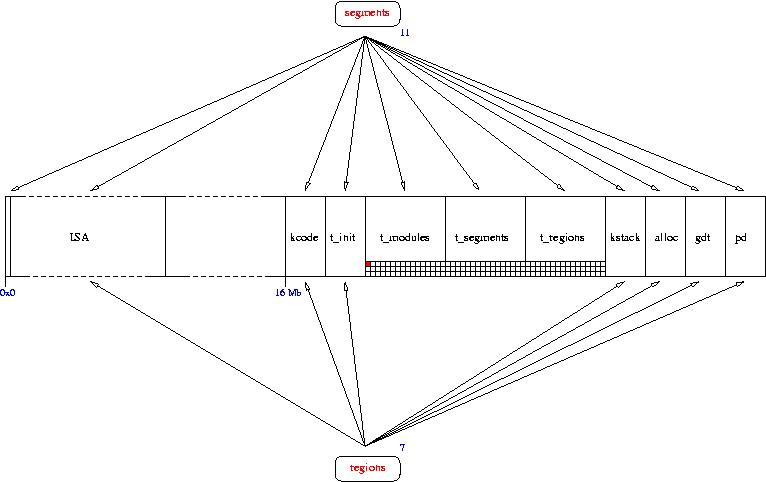
\includegraphics[scale=0.5]{figures/k1-memory-layout.jpg}}
\end{figure}

All the segments must be mapped at the kernel boot time.

Be careful to correctly initialise the machine-dependent fields
including \textit{gdt} and \textit{pd} which will be used by the microkernel
to retrieve the structures in main memory.

%
% k2
%

%
% k3
%

%
% k4
%

%
% k5
%

%
% kn
%



\end{document}
